%This is the third chapter of the dissertation

%The following command starts your chapter. If you want different titles used in your ToC and at the top of the page throughout the chapter, you can specify those values here. Since Columbia doesn't want extra information in the headers and footers, the "Top of Page Title" value won't actually appear.
\pagestyle{plain}


\chapter[Cascaded Silicon Photonic Ring Resonators Architecture for Reconfigurable WDM Applications][Top of Page Title]{Programmable Cascaded Microring Resonators for Reconfigurable WDM Applications}

\textit{\textbf{Abstract -} In this chapter we introduce a widely used architecture of cascaded microring resonators that share a common waveguide bus. Based on the photonic design, we develop a power-aware algorithm on an FPGA platform that controls the spectral responses of the microrings to enable optical unicast, multicast and broadcast of WDM signals. The system demonstration consists of an optically and electrically packaged SiP chip with an array of eight microrings and a fast tunable C-band laser delivering programmable wavelength and spatial switching capabilities.}

\textit{We characterize the thermo-optic response of microring resonators and extract key parameters necessary for the development of the control-plane. The performance of the proposed architecture is tested with 10 Gb/s data rate and error-free operation is verified for various switching scenarios. Based on the tuning efficiency, electrical power and energy consumption is determined to reconfigure the SiP chip in the ITU grid for all possible wavelength operations and output ports combinations and show that unicast, multicast of two, three, four, five, six, seven, and broadcast functions are achieved with energy overheads of 0.02, 0.07, 0.18, 0.49, 0.76, 1.01, 1.3, and 1.55 pJ/bit, respectively.}

\textit{Utilizing the system, we further expand the control algorithm to demonstrate a programmable optical power distribution functionality. The abstraction of the physical layer allows to achieve precise power profiles profiles from the drop ports of the MRRs.}

\section{Introduction}

Today's DCs are experiencing an unprecedented increase in network traffic due in particular to the popularity of video streaming services and cloud-based computing \cite{hashem2015rise}. Server and network virtualization further exacerbate the trend \cite{wang2010impact}. This creates bottlenecks in data movement between DCs racks and processing workloads inside the rack. To address this high demand, new network architectures are proposed to provide bandwidth and resource allocation \cite{wen2016flexfly} for intra \cite{yan_FPGA_DC} and inter  \cite{kachris2012survey,bergmanoptical} racks through reconfigurable optical interconnects. These architectures, including Proteus \cite{singla2010proteus} and MORDIA \cite{farrington201310,aguinaldo2014energy}, achieve flexible networking through optical spatial switching \cite{farrington2012demonstration} or optical wavelength switching \cite{zhang2012experimental}, and augmented with optical multicasting \cite{samadi2015optical,brunina2011building}.  

In spatial switching, data carried on an optical carrier is deflected to any of the of the output ports in a configurable way. The term spatial is used to underline the fact that only the spatial routing of the light is modified. In wavelength routing, in contrast, received optical signals can be further decomposed in wavelengths, and the propagation direction of each of these wavelengths can be separately configured. Finally, in optical multicasting, incoming optical signals can simultaneously be forwarded to more than one output ports simultaneously \cite{chen2011survey}.

Most of the deployed optical switches, however, rely on discrete optical elements such as micro electro-mechanical systems (MEMS) actuated micro-mirrors arrays or Liquid crystal on silicon (LCOS) matrices \cite{robertson2014demonstration,hamza2016free,wavelength2016}. The individual cost of these elements, and sometimes their bulkiness and mechanical susceptibility, is a severe hindrance to a high utilization in large scale interconnects. To be widely deployed in datacenters as in other systems involving large data exchanges, compact, power-efficient, and above all, scalable switches are required. Silicon photonics (SiP) has emerged over the last decade as a platform for development of photonic integrated circuits (PICs) \cite{komljenovic2016heterogeneous,alloatti2015photonics}. Thanks to the utilization of already available advanced silicon based CMOS electronics foundries to fabricate and package PICs \cite{novack201330,leemeeting,bogaerts2005nanophotonic}, SiP inevitably enables significant cost reductions at scale while chip-level integration guarantees compactness. Numerous SiP integrated components have been implemented ranging from passive wavelength splitters and filters to active modulators and switches \cite{lu201616,biberman2011broadband,subbaraman2015recent}. To orchestrate these many individual SiP devices within a full network, however, a unified control plane is required \cite{calhoun2016hardware,chen2015programmable} to set the proper command signals. 

In 2011, Xu \textit{et al.} \cite{xu2011hybrid} demonstrated a SiP-based hybrid optical wavelength selective switch (WSS) platform that can potentially be utilized in data centers. The demonstrated WSS was a 1$\times$2 switch based on SiP microring resonators and showed error free performance for both OOK and DPSK optical modulation. However, a comprehensive control plane architecture to control silicon photonics and external components was not demonstrated in this work. In 2014, Calhoun \textit{et al.} \cite{calhoun2014dynamic} discussed the importance of the capability of silicon photonic switches in terms of dynamic configurability. They used 2$\times$2 broadband SiP Mach-Zehnder switch and a 1$\times$2 WDM demultiplexer based on microring resonators. Quite interestingly, this work focused on a unified control plane to orchestrate the photonic devices side-by-side. However, the demonstrated system still lacked to portray a picture of how the control plane would evolve if the system scales up and did not support routing of complex patterns such as multicast. 

In this chapter, we describe a system based on a common array of cascaded microring resonator (MRR) in the form of a packaged SiP chip, connected to an external Y-branch fast tunable laser \cite{browning2013optical}. The control over the SiP chip and the laser is developed on an FPGA platfrom and abstracted into a single programmable command. The control algorithm is optimized to achieve minimum energy consumption due to thermal control \cite{biberman2008thermally} of the SiP chip for all possible wavelength and spatial switching scenarios. To the best of our knowledge, it is the first time that a control plane capable of performing optical multicast in SiP platform utilizing a single wavelength source is demonstrated. In the experimental demonstration we examine the transmission quality of incoming 10Gb/s OOK signals in terms of eye-diagram and BER from unicast to broadcast of eight at various operational wavelengths. 

In the last section of the chapter, we further expand the control algorithm to demonstrate a programmable optical power distribution using the same system architecture. First, a motivation for such functionality is presented and then experimental results of precise power profiles are shown within several percent error margin from the programs input.

\section{System architecture and functionality}


Figure \ref{fig1} shows a block diagram of the proposed system architecture. The main components are a fast tunable laser (TL), a SiP chip, two field programmable gate arrays (FPGAs) and a computer that provides an interface to the user. Depending on the desired configuration, the computer sends operation messages to the two FPGAs via a serial data transfer interface. One FPGA translates the messages into command signals for the TL to adjust its output optical power and the wavelength of operation over the C-band. The other FPGA controls the spectral responses of an array of eight cascaded MRRs. As shown in Fig. \ref{fig1}, an external modulator is used to encode data onto the laser output. Through software abstraction of the physical layer, the system is capable routing incoming optical data to any of the eight output ports, as well as splitting the incoming data (multicasting) to a number of output ports by precise and predetermined control voltages on each MRR. 

\begin{figure}[b]
\begin{center}
\includegraphics[width=13cm]{Chapter3/fig1.pdf}
\caption{Block diagram of the system including a tunable laser, SiP device, and two control FPGAs. The data modulates the laser's wavelength and is transmitted through the SiP device. The central control computer can reconfigure the tunable laser and the SiP device to switch the data to any number of the eight ports (a), wavelength routing (b), and multicasting (c).}
\label{fig1}
\end{center}
\vspace{-0.9cm}
\end{figure}

The time-slot diagram in Fig. \ref{fig1} illustrates three possible operation of the system. In this example, the different colors of the \textit{Data} in the figure correspond to different wavelengths of the TL. During slot $\Delta t_0$ the data stream is routed to output R1. In between $\Delta t_0$ and $\Delta t_1$ slots the data stream is switched to output R4  (Fig. \ref{fig1}(a)) without changing the operating wavelength (red color). In the second case, shown in Fig. \ref{fig1} (b), wavelength routing is performed. During time slot $\Delta t_2$ the data is transmitted to output R2 on a carrying wavelength $\lambda_1$ (green color) while in slot $\Delta t_3$ the output port stays the same but the wavelength changes to $\lambda_2$ (blue color).  Finally, a multicast (one to many) operation is shown in Fig. \ref{fig1}(c). During slot  $\Delta t_4$, an incoming data stream modulated on a user's chosen wavelength (purple color) is split among four output ports: R2, R4, R7, and R8.  In the following time slot  $\Delta t_5$, the recipients of the multicast operation are modified to R1, R3, R5, and R6. The transition time between the time slots is determined by the reconfiguration time of either the TL ($\sim$ 10 ns \cite{browning2013optical}) or the SiP device ($\sim$ 20 $\mu$s) from the moment the FPGAs apply the command signals.

The operation of the system is not limited to the particular sequential illustration presented in Fig. \ref{fig1}.  Because the TL can operate at 40 distinct wavelength channels in the C-band ITU grid, and the SiP device can perform unicast (one to one), multicast (one to many), and broadcast (one to all) operations, numerous deterministic combinations are possible without any constraints. 

\section{SiP control plane}

\begin{figure}[t]
\begin{center}
\includegraphics[width=13cm]{Chapter3/fig2.pdf}
\caption{(a) Measured thermo-optic response of the heater-ring system of the eight rings. Inset illustrates a schematic of the SiP device where each MRR has its own individual resistive heating element. (b) Averaged shift of resonance as a function of dissipated power in eight rings. Bottom inset illustrates a red shift and the top inset shows the measured 3dB bandwidth of each drop port.}
\label{fig2}
\end{center}
\vspace{-0.9cm}
\end{figure}

%%%%%%%%%%%%%%%%%%%%%%%%%%%%%%%%%%%%
%\textbf{Through integration of micro-heater on top of each MRR, the large thermo-optic coefficient of silicon \cite{komma2012thermo} can be leveraged to precisely control the rings' spectral responses. Although precise, thermal control is limited to the micro-second \cite{atabaki2010optimization} regime in our demonstration. Faster control could be achieved by injecting or depleting charge carriers into/from the silicon waveguides to control the resonance \cite{wu2015compact}. The proposed architecture relies on the fast tunable laser with nano-second timescale reconfiguration \cite{browning2013optical} in order to bypass the slower thermal response of the SiP MRRs. Nevertheless, the reconfiguration of the SiP device is required whenever multicast functionalities and broadcast are demanded. }
 
To obtain reliable reconfigurability of the packaged SiP device, a characterization of the dynamic behavior of each MRR must be performed. The MRRs are designed with varying radii around 7$\mu$m enabling different wavelengths of operation when no bias is applied. The inset of Fig. \ref{fig2}(a) shows a schematic of the SiP chip where each MRR has an electrical interface to a resistive heating element fabricated on top \cite{atabaki2010optimization}. Due to the high thermo-optic coefficient of silicon \cite{komma2012thermo}, an increase in the supplied voltage to the heater increases the local temperature of the ring and causes a change in the effective index of the optical mode allowing the resonance of the rings to shift to higher wavelengths (red shift). To achieve accurate and error-free switching operations, the thermo-optic response (shift of resonance vs. applied voltage) of each individual ring is measured and stored in the control plane. To that end, the optical signal is coupled to and from the chip through an aligned and glued fiber-array directly on top of the embedded grating coupler structures. Fig. \ref{fig2}(a) shows normalized responses as a function of increased bias voltage. Second order polynomial functions have been fitted to the measured results allowing a continuous and accurate relationship between the supplied bias voltage and the frequency response. These functions together with MRRs' Lorentzian resonant response \cite{bahadori2016comprehensive} (e.g. 3 dB bandwidth of 87 GHz shown in the inset Fig. \ref{fig2}(b)) and zero bias resonances are used in the control algorithm to perform any type of switching operation.
 
\begin{figure}[b]
\begin{center}
\includegraphics[width=13cm]{Chapter3/fig3.pdf}
\caption{(a) Illustration of the spectral response of the chip with zero bias. (b) Illustration of the spectral response of the chip in unicast operation. (c) Demonstration of a detuning procedure where 10Gbps data is modulated on wavelength  1543.09 and both MRR 2 and 8 are tuned to the same resonances. (d) Illustration of the spectral response of the chip in multicast operation.}
\label{fig3}
\end{center}
\vspace{-0.9cm}
\end{figure}

In addition, the electrical power dissipated by the heaters as a function of the resonance shift is shown in Fig. \ref{fig2}(b). A slope of 0.266 nm/mW defines the tuning efficiency. We utilize this parameter to estimate the range of the required power overhead (minimum and maximum) to perform all possible switching cases (unicast, multicast, and broadcast).

\subsection{Unicast, multicast and broadcast functionalists}

In order to achieve different data routing operations, the TL, via its control FPGA, is set to the desired transmission wavelength, while the SiP chip's control FPGA is instructed to supply bias voltages necessary to shuffle spectral responses based on the chosen data routing operation. Figure \ref{fig3}(a) illustrates the responses of the MRRs in our chip when no bias voltage is applied. By design, the responses of the rings are separated by 1.27 nm ($\sim$ 160 GHz) with an FSR of 13 nm and 3 dB bandwidth of 0.7 nm.

-->>I AM HERE<<--

Figure \ref{fig3}(b) shows a unicast operation where the input data on the wavelength denoted by a red vertical arrow is routed to output port 8 (dashed black curve). To obtain this mode of operation, i) the resonance of ring R2 must be detuned to prevent dropping at port 2 because R2 has the precedence over R8 in the MRR array, and ii) the resonance of ring R8 must be tuned to the red wavelength. The amount of detuning required for ring R2 to achieve error free operation is obtained experimentally and demonstrated in Fig. \ref{fig3}(c). As the bias voltage over R2 is increased gradually, its resonance is shifted to allow the signal to propagate to R8. The bit-error-rate (BER) and the eye-diagrams are captured at output port of R8 to verify the amount of detuning necessary in order to reach the error free transmission (BER = 10$^{-12}$) with negligible crosstalk effects \cite{bahadori2016crosstalk}. At a bias of 0.85 V the signal is fully routed to the output port 8. We estimated that this amount of detuning is about 1.08 nm which corresponds to a channel suppression of 10 dB between the desired output port (R8) and the detuned MRR (R2). This amount of detuning is chosen for power efficiency; any further detuning will cost more energy-per-bit while introducing negligible improvement on the BER of the routed 10 Gbps OOK signal. 

Figure \ref{fig3}(d) illustrates a one-to-seven multicasting operation. This operation is possible by aligning the Lorentzian response of each MRR so that the power of the optical signal is divided equally among the desired output ports; i.e. tuning the rings to the appropriate resonances, starting from the last MRR participating in the multicast operation. The last MRR, R8 in this example, is tuned so that its resonance aligns exactly with the TL wavelength, allowing maximal transmission over its drop path. R7 is then tuned to its 3dB bandwidth point, allowing a drop of 50\% of the optical power. Continuing with this approach R6, R5, R4, R3 and R2 are tuned to the following drop power ratios: 33.33\%, 25\%, 20\%, 16.67\% and 14.28\%, respectively, i.e. following a harmonic series (1, 1/2, 1/3, 1/4 $\dots$). When the process is complete, each of these seven rings will equally drop 14.28\% of input optical power coupled into the SiP chip. Realizing multicast exhibits the fine tuning levels our system is capable of, and demonstrates the potential of SiP for error-free multicast operation of one stream of data over a single wavelength.


%****************************
\subsection{Software implementation }

Once the SiP device is fully characterized, collected measurement data can be exploited by an algorithm to find the ideal device settings corresponding to a specific configuration.

\begin{figure}[b!]
\begin{center}
\includegraphics[width=13cm]{Chapter3/fig4.pdf}
\caption{(a) The flowchart of the control algorithm to achieve optimal tuning. (b) If the laser wavelength is located outside the two possible tuning points (A and B), point A is selected. (c) If the laser falls between the A and B tuning points, point A is not accessible. Therefore, point B is targeted as it requires less tuning power than point C or D.}
\label{fig4}
\end{center}
\vspace{-0.9cm}
\end{figure}

The flowchart in Fig. \ref{fig4}(a) describes our algorithm to configure the SiP chip for all possible switching cases. We implemented the algorithm in a host computer in Python and post calculation commands are sent to the two FPGAs that control the TL and the SiP device, respectively.



The algorithm takes two arguments. The first is channel number, which determines the wavelength of operation for TL, and the second argument is a binary array indicating where to route the signal. For example, \textit{set\_switch(ch1,[0,1,0,0,0,0,0,0])} will route the input data on wavelength $\lambda_1$  to output port R2 and \textit{set\_switch(ch2,[0,1,0,1,1,1,1,1])} will perform a multicast of the input data on wavelength $\lambda_2$  to output ports R2, R4, R5, R6, R7 and R8. The resonance of the MRR corresponding to the last selected port is always tuned exactly to the selected channel in order to provide a 100\% drop of power. The resonance of the next selected port will be set to achieve 50\% drop and so forth. For the unselected ports, our software executes an adaptive detune operation in which it determines if the MRR needs to be shifted from the 10 dB region or can be left untouched. After the main loop is completed, the amount of the required wavelength shifts for the MRR array are converted to corresponding bias voltages and sent to the control FPGA of the SiP device.

Due to the symmetrical spectra of the MRRs it is possible to drop the required amount of optical power from either side of the Lorentzian response. To optimize the tuning power consumption of the MRR array the software automatically selects the closest tuning option. Fig. \ref{fig4}(b) shows the case where the laser (red arrow) is outside of the two possible tuning points (markers A and B). After the execution of the algorithm, the nearest point (A) is aligned with the laser. Figure \ref{fig4}(c) depicts the case where the laser wavelength falls in between the two possible operation points (markers A and B). In this example, the MRR will be shifted to the left, to align with point B. Note that in this case the point on the right side of the laser (marker A) is not accessible due to the red-shift nature of thermal tuning. Using the two sides of the Lorentzian response, in this particular case, avoids reaching point C, which requires a large heater power. 


%%%%%%%%%%%%%%%%%%%%%%%%%%%%%%%%%%%%%%%%%%%%%%%%%%%%%%%%

\section{Experimental demonstration and evaluation}

The schematic of the experimental setup is shown in Fig. \ref{fig5}. A tunable Y-branch laser \cite{browning2013optical} (Fig. \ref{fig5}(a)) mounted on an FPGA board was used to output light at various frequencies across the ITU 100 GHz C-band grid. The packaged SiP device along with its control plane is shown in Fig. \ref{fig5}(b). The control plane is based on an Stratix III EP3SL150 FPGA (separate from the laser) capable of hosting and controlling eight parallel digital-to-analog converters (65 MHz DAC) with 14 bits of resolution. An image of the DACs mounted on top of the FPGA is marked by (1) in Fig. \ref{fig5}(b). The output voltage from the DACs (0--1 V) is amplified by 5 in the gain stage (marked as (2)) to achieve a full FSR swing for each MRR. The amplified control signals are connected to a break-out printed-circuit-board (PCB) (marked as (3)) which hosts the SiP chip. After fabrication, the chip was attached to, and wire-bonded on, a standard electrical IC package (marked as (4)). The silicon photonic chip used in this work is not equipped with any temperature sensors, so no active temperature stabilization procedure is included in the design of the chip. However, the chip is sitting on a heat sink in the IC package that passively regulates its temperature to the ambient temperature level. An array of optical fibers is glued to the packaged chip on top of grating couplers (marked as (5)). 

\begin{figure}[t!]
\begin{center}
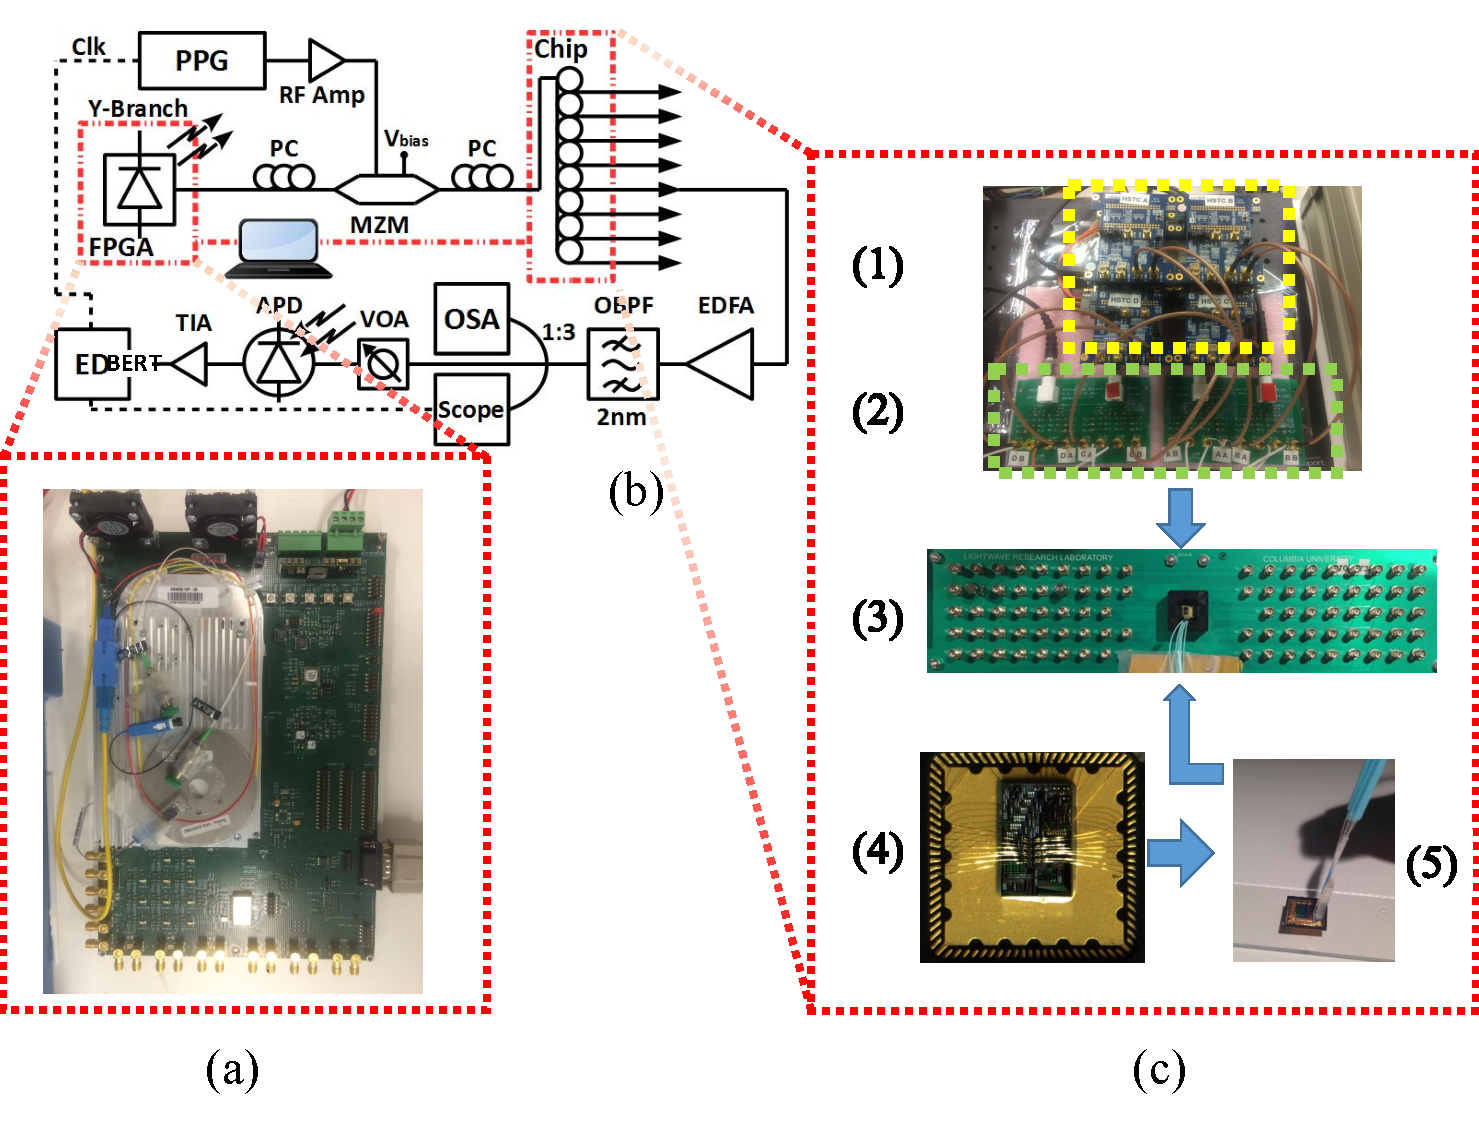
\includegraphics[width=13cm]{Chapter3/fig5.pdf}
\caption{(a) An image of a fast, C-band tunable laser. (b) Schematic of the experimental setup. Pulse Pattern Generator (PPG), Erbium Doped Fiber Amplifier (EDFA), Mach Zehnder Modulator (MZM), Bit Error Rate Detector (BERT), Avalanche Photodiode (APD), Trans-Impedance Amplifier (TIA), Variable Optical Attenuator (VOA), Polarization Controller (PC), Optical Spectrum Analyzer (OSA), Optical Bandpass Filter (OBPF). (c) Packaged SiP device with its control plane: (1) four dual DAC cards on an FPGA development board, (2) electrical Gain stage (3) breakout PCB (4) packaged and wire-bonded SiP (5) An array of ten fibers glued on the SiP chip. }
\label{fig5}
\end{center}
\vspace{-0.9cm}
\end{figure}

To test various switching scenarios, a PPG was used to output a 10 Gbps PRBS (2$^{31}$-1) signal, which was then electrically amplified before being modulated onto the optical carrier using a Mach-Zehnder modulator. The optical signal was then sent to the SiP device, configured through the software control plane, to route the signal to the desired output port(s). Because the SiP chip exhibits coupling loss of $\sim$ 25 dB due to its packaging, in our experiment an EDFA was required to amplify the received signal. Using a 1:3 divider, the optical signal was directed to an OSA, an oscilloscope to observe the received eye diagram and an APD. The power falling on the APD was kept at a constant level of -8 dBm to avoid saturation. The output of the photo-receiver was sent to the bit error rate tester (BERT) for BER measurement. The BERT and oscilloscope were both triggered with the same clock signal from the PPG.


%****************************
\subsection{Unicast}

Figure \ref{fig6} maps all possible unicast combinations based on wavelength and spatial routing capabilities of the system. The spatial ports are denoted in the vertical axis where MRR 1 corresponds to the first output port in the cascaded topology. The horizontal bars illustrate the tuning range of each MRR with a zero bias resonance at the grey vertical lines. The thin vertical dashed lines separated by 100GHz correspond to the all possible optical channels of the TL. The thicker dashed lines and the eye-diagrams to their right indicate the TL channels and the drop port combinations which were used in our experiment. 

A 10Gbps optical signal was injected into the input port of the chip and various wavelength routing and spatial switching configurations were tested in order to confirm error-free operation (in these cases all measured BER $\leq$ 10$^{-12}$) operation. The control plane was first set to test spatial switching, where data carried on a specific wavelength was switched from one drop port to another. The TL laser was set to channel 22 (1541.70 nm) and the signal quality (Eye diagram and BER) was monitored over four different switching cases for drop ports of MRRs 1, 2, 3 and 4. Similarly, The TL was set to channel 13 (1551.28 nm) and the control plane configured the SiP for four different cases to route the data to the output ports 5, 6, 7, and 8. 

Next, wavelength routing was tested where the data is routed through a specific port, each time with a different wavelength. The eye-diagram and BER were captured at port R1 while the control plane reconfigured the transmitted wavelengths to 1533.81 nm, 1537.75 nm, 1541.70 nm, and 1549.67 nm. In a similar measurement, the signal quality was measured at port R8 with the following wavelengths: 1529.12 nm, 1543.29 nm, 1551.28 nm, and 1560.97 nm.

The results of this part of our experiment demonstrate the capability of the SiP-based system for error-free optical unicast operation.


%****************************
\subsection{Multicast and broadcast}

\begin{figure}[t!]
\begin{center}
\includegraphics[width=13cm]{Chapter3/fig6.pdf}
\caption{Tuning ranges of eight cascaded MRRs in the C-band. The eye-diagram plots are captured from experimentally tested error-free unicast operation at various combinations of wavelength and output ports. Color strips are used to differentiate the outputs. }
\label{fig6}
\end{center}
\vspace{-0.9cm}
\end{figure}

Figure \ref{fig7} shows experimental measurements for multicast and broadcast operations, and the best and worst power consumptions for each operation. All the results were set to perform at channel 17 of the laser (1548.11 nm). First, the control plane was set to route the data to R2. Then the SiP device was reconfigured to multicast the data to ports R2 and R7. The BER and the eye-diagrams were captured at the two output ports separately to verify error-free operation. This process continued to higher multicast port counts until it covered all the eight ports (broadcast). The tested multicast cases are marked by eye-diagram results in each row of Fig. \ref{fig7}. 

\begin{figure}[t!]
\begin{center}
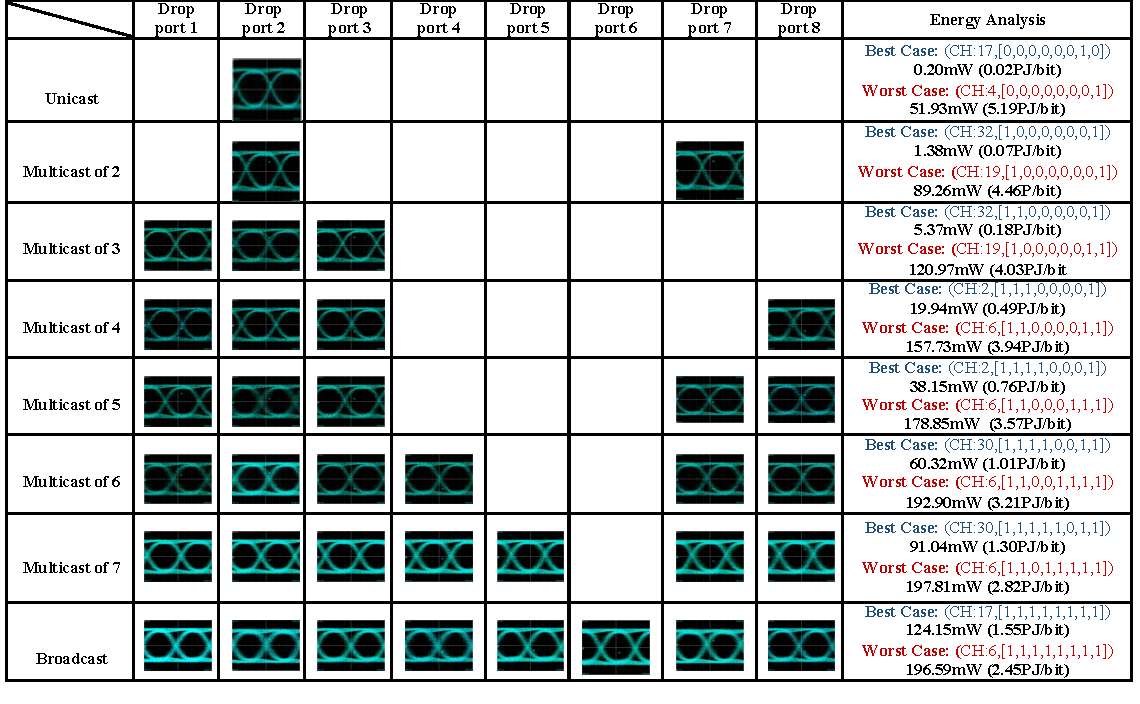
\includegraphics[width=13cm]{Chapter3/fig7.pdf}
\caption{Experimental results of 8 different cases including Unicast, Multicast and Broadcast operated at 1548.11nm are shown in first 8 columns. The last column shows the estimation of best and worst case power consumption for all possible configurations. }
\label{fig7}
\end{center}
\vspace{-0.9cm}
\end{figure}

The column on the right side of Fig. \ref{fig7} shows power overhead analysis due to the reconfiguration (thermal tuning) of the SiP device. All possible combinations of TL wavelengths and SiP output ports were swept in order to determine the best and the worst case of power consumption. The results were achieved by estimating the amount of wavelength shift (in nm) necessary for each MRR, converting it to ohmic power (in mW), and summing them up to get the overall mW consumption. With a data rate of 10 Gbps, the static ohmic power of each participating MRR was also converted to energy per output-bit (pJ/bit) overhead. Finally, the total pJ/bit was obtained by adding all the individual pJ/bit values.

For example, for multicast using 3 ports, the best power consumption is calculated to be 5.37 mW for the \textit{(ch32,[1,1,0,0,0,0,0,1])} combination with an energy overhead of 0.18 pJ/bit. While the worst combination is \textit{(ch19,[1,0,0,0,0,0,1,1])} resulting in an ohmic power of 120.97 mW and an energy overhead of 3.94 pJ/sent-bit (1.31 pJ/received-bit).

\section{Programmable optical power distribution}

Building on the multicasting algorithm, we expand the control plane over the SiP cascaded MRRs to perform programmable optical power distribution. This capability can pave the way for future optical network requirements that focus on higher utilization and reduced energy consumption. 

Since the quality of transmission (bit error ratio, BER) in a digital optical links is directly related to the optical signal-to-noise ratio, pumping more optical power into a communication link will result in a better reception of the data as long as the optical power is kept below the nonlinearity threshold of the transmission medium \cite{bahadori2015nonlinear}. Additionally, the distribution of optical power can be further optimized for bandwidth and/or distance requirements of each point-to-point link \cite{ramaswami2009optical}. Optical power distribution has also the potential to reduce energy consumption in optical networks with a centralized optical source. A single high-power laser is known to achieve more than 40\% of efficiency \cite{heck2014energy} and can be utilized as an external central power source in conjunction with a dynamic power allocation routines \cite{posca2018powering}. 

To execute the programmable optical power distribution we again utilize the parameters necessary to fit the Lorentzian function describing the spetrcal response of each MRR: resonance wavelength and 3dB bandwidth as shown in Fig. \ref{fig2}. Together with the dynamic thermo-optic responses we obtain the optical drop power as function of the applied bias voltage (DR(V)). This functions are saved in the FPGA as a look-up table.

The power distribution functionality is abstracted into a single command called \textit{set\_power}($\lambda$, power, [$\alpha_1$,$\alpha_2$,$\alpha_3$,$\alpha_4$,$\alpha_5$,$\alpha_6$,$\alpha_7$,$\alpha_8$]) 
set by the user in the processor core of the Altera FPGA (nios-ii). The input entries $\lambda$ and power control the TL \cite{browning2013optical} to the desired wavelength and power in dBm units, and $\alpha_1$ to $\alpha_8$  ($\sum_{i=1}^{8}\alpha_i \leq 1$)  set the desired drop ratios from output ports 1 to 8. Due the cascaded design of the SiP chip, the user input ratios are converted to power drops based on the following relationship:
\begin{equation}\label{CH4_eq2}
DR_1 = \alpha_1, DR_i = \frac{\alpha_i}{1-\sum_{1}^{j-1}\alpha_j}
\end{equation}
As an example, for equal power distribution through the first four ports ($\alpha_1=\alpha_2=\alpha_3=\alpha_4=25 \%$) the actual programmed drop levels are set to $DR_1= 25\%$ , $DR_2= 33.3\%$, $DR_3= 50\%$, $DR_3= 100\%$ based on Eq. \ref{CH4_eq2}. The calculated drop ratios of the participating ports are translated to bias voltages, and if one of the non-participating ports’ spectral response lines up with the wavelength of operation, it is automatically de-tuned from its zero-bias operation (as shown in Fig. \ref{fig3}(b)). The optical coupling variation between the ports and the fibers is calibrated and taken into account to further increase the accuracy of the algorithm. 

\begin{figure}[t!]
\begin{center}
\includegraphics[width=13cm]{Chapter3/CH_3_power_dis.pdf}
\caption{Demonstration of dynamic power distribution through drop-ports of cascaded microring resonators (a) Equalized power distribution for four rings. (b) Power down and up for four rings. (c) 3dB step up for three rings. (d) Power up and down for three rings. Note that the wavelength of operation is different for each case and is set by the user.}
\label{fig8}
\end{center}
\vspace{-0.9cm}
\end{figure}

Figure \ref{fig8} summarizes the experimental results of four distinct distribution profiles at different operating wavelengths and 12dBm of laser power. Fig. \ref{fig8}(a) shows the results for equalized power profile [1/4,1/4,1/4,1/4,0,0,0] among ports 1, 2, 3 and 4 at 1530.7nm, and Fig. \ref{fig8}(b) shows [0,0,0,1/3,1/6,  1/6,1/3] profile at 1551.31nm. Fig. \ref{fig8}(c) corresponds to a ramp-up profile set to [1/7,0,2/7,0,4/7,0,0] at 1543.331nm and Fig. \ref{fig8}(d) corresponds to a mixed profile of [0,1/3,0,1/2,0,1/6,0] at 1555.35nm. The corresponding applied bias voltage array for each case are [0.97, 0.80, 1.77, 2.35,0,0,0] V, [0,0,0.48, 0.80, 1.15, 1.70, 2.3] V, [1.04,2.00,1.65,0,2.94,0,0] V and [1.04,0.90,0,2.06,0,3.09, 0] V respectively. For cases 3(b)-(d), it can be seen that bias voltages are applied to more MRRs than participating ports in the power profile. The additional MRRs are the ones that need to be de-tuned from their zero-bias operation. These results show the capability of the system to generate wavelength selective power profiles within several percent error margin from the programmed input. 









%%%%%%%%%%%%%%%%%%%%%%%%%%%%%%%%%%%%%%%%%%%%%%%%%%%%%%%%
\section{Conclusion}

For the first time, we demonstrate a fully integrated software control plane in order to realize optical unicast, multicast and broadcast in conjunction with wavelength selectivity on a silicon photonic chip.  We show that any switching configuration set by the user input could be precisely determined in an energy efficient way by our control plane. This level of abstraction of the physical layer paves the way for directly integrating SiP-based devices into a higher-level control plane under a software defined networking (SDN) paradigm. SDN and all optical routing are key requirements for next generation reconfigurable optical networks/interconnects.

Based on the static spectral response and thermo-optic behavior or silicon-based microring resonators, a control plane was developed to dynamically distribute the optical power to the drop ports of an array of seven add-drop ring resonators. We demonstrated, experimentally, various power profiles including uniform, ramp up, and mixed based on the predicted heater voltages in the control plane. 